\chapter{Use Case 2: FixMyStreet}

\section{Einführung}
FixMyStreet ist ein Konzept, welches bereits in verschiedenen Städten bzw. Ländern umgesetzt wurde. Beispiele dafür sind Deutschland welches dazu die Webseite  \url{http://de.seeclickfix.com/} anbietet oder England mit der Webseite \url{http://www.fixmystreet.com/}. Beide Beispiele bieten neben der Webseite auch eine native App für iOS und Android an.

Die Idee hinter dem Konzept ist so einfach wie auch genial. Man ermöglicht dem Bürger per Webseite oder App entdeckte Defekte in seiner Umgebung (defekte Strassenlampen, Schlaglöcher, usw.) direkt der Stadt oder Gemeinde zu melden. Diese kann dann diese Meldungen überprüfen und wenn nötig beheben. So können teure Kontrollfahrten auf ein Minimum reduziert werden.

\subsection{Ziel}
Das Ziel dieses UseCases war die Erstellung einer WebApp, welche genau dieses Konzept umsetzt. Die Benutzer sollen die Möglichkeit haben Defekte in ihrer Umgebung dem zuständigen Amt zu melden.

Google Fusion Table soll dazu als Datenbank verwendet werden, in der die Defekte abgelegt werden. Natürlich sollen auch einige GIS-Features der Fusion Table verwendet werden, um beispielsweise nur die Defekte im aktuell sichtbaren Bereich der Karte zu laden.

\section{Anforderungsspezifikation}
\subsection{Use Cases}
\begin{figure}[!h]
	\centering
	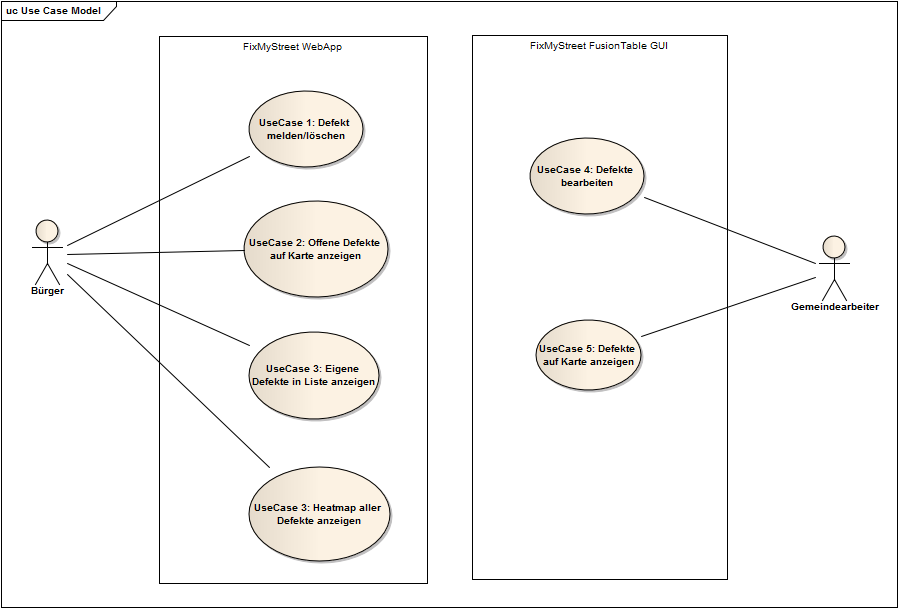
\includegraphics[scale=0.5]{images/usecase2-fixmystreet/fixmystreet-usecasediagram.png}
	\caption{FixMyStreet UseCase Diagramm}
	\label{fixmystreet-usecasediagram}
\end{figure}

\subsubsection{Use Case 1a: Defekt melden}
\paragraph{Primary Actor}
\begin{itemize}
\item Bürger
\end{itemize}

\paragraph{Stakeholders and Interests}
\begin{itemize}
\item Bürger: Möchte einen entdeckten Defekt melden
\end{itemize}

\paragraph{Preconditions}
\begin{itemize}
\item WebApp ist gestartet
\end{itemize}

\paragraph{Success Guarantee (Postconditions)}
\begin{itemize}
\item Neuer Defekt ist in Datenbank gespeichert
\item Defekt ist in der Liste und auf der Karte ersichtlich
\item Melde-Maske wurde in den Ursprungszustand zurückgesetzt (kein Defekttyp ausgewählt, Markierung wieder auf die aktuelle Position verschoben)
\end{itemize}

\paragraph{Main Success Scenario}
\begin{enumerate}
\item Bürger wählt Defekttypen aus
\item Bürger verschiebt Markierung auf Karte zur Position des Defekts
\item Bürger sendet den Defekt ab
\item Bürger bestätigt die Kontrollfrage, ob der defekt tatsächlich gesendet werden soll
\end{enumerate}

\paragraph{Alternative Flows}
2a. Markierung muss nicht zwangsläufig verschoben werden. Sie zeigt beim Starten der WebApp auf die aktuelle Position. Falls dies nicht zugelassen wird zeigt sie auf einen vorkonfigurierten Ort.

\paragraph{Special Requirements}
-

\paragraph{Frequency of Occurrence}
Tritt sehr häufig auf, da eine beliebige Anzahl von Bürgern Defekte melden kann.

\subsubsection{Use Case 1b: Defekt löschen}
\paragraph{Primary Actor}
\begin{itemize}
\item Bürger
\end{itemize}

\paragraph{Stakeholders and Interests}
\begin{itemize}
\item Bürger: Möchte einen bereits gemeldeten Defekt löschen
\end{itemize}

\paragraph{Preconditions}
\begin{itemize}
\item WebApp ist gestartet
\item Die Listenansicht wurde geöffnet 
\item Es wurde bereits ein Defekt gemeldet
\end{itemize}

\paragraph{Success Guarantee (Postconditions)}
\begin{itemize}
\item Der Defekt wurde aus der Datenbank gelöscht
\item Defekt ist nicht mehr auf der Liste und auf der Karte ersichtlich
\end{itemize}

\paragraph{Main Success Scenario}
\begin{enumerate}
\item Bürger markiert den zu löschenden Defekt in der Liste
\item Bürger wählt den Befehl \emph{Löschen}
\end{enumerate}

\paragraph{Alternative Flows}
2a. Falls der Status des Defektes bereits von einem Gemeindearbeiter geändert wurde, ist es für den Bürger nicht mehr möglich den Defekt zu löschen.

\paragraph{Special Requirements}
-

\paragraph{Frequency of Occurrence}
Tritt sehr häuft auf, da es für jeden Bürger, welcher bereits einen Defekt gemeldet hat, möglich ist seine eigenen Defekte wieder zu löschen.

\section{Analyse}

\section{Design}

\subsection{ERD}

\subsection{Klassendiagramm}

\section{Implementation}
\subsection{Systemanforderungen:}
Die WebApp basiert auf dem Sencha Touch 2 Framework. Dieses bietet eine Basis zur Erstellung von mobilen WebApps mit JavaScript. Das Sencha Touch 2 Framework unterstützt alle WebKit-fähigen Browser:

\paragraph{Desktop:}
\begin{itemize}
\item Chrome
\item Opera
\item Safari
\end{itemize}

\paragraph{Mobile:}
\begin{itemize}
\item iOS
\item Android
\item Blackberry
\end{itemize}

\subsection{Abhängigkeiten}
\begin{tabular}{|l|l|}
\hline 
Library & Version \\ 
\hline 
Sencha Touch 2 & 2.0.1 \\ 
\hline 
jQuery & 1.7.1 \\ 
\hline 
Google Maps API & V3 \\ 
\hline 
gftlib-js & 1.0 \\ 
\hline 
\end{tabular} 

\section{Implementation}
\subsection{Quellcode-Struktur}
\begin{tabular}{|l|l|}
\hline 
Datei & Beschreibung \\ 
\hline 
resources/images/ & Bilder der Applikation \\ 
\hline 
resources/styles/ & CSS-Styles der Applikation \\ 
\hline 
app/app.js & Einstiegspunkt der Applikation \\ 
\hline 
app/controller/List.js & Kontroller der \emph{List}-View \\ 
\hline 
app/controller/Map.js & Basis-Kontroller der \emph{Report}-View und der \emph{Map}-View \\ 
\hline
app/controller/ProblemMap.js & Kontroller der \emph{Map}-View \\ 
\hline
app/controller/ReportMap.js & Kontroller der \emph{Report}-View \\ 
\hline
\end{tabular} 

\section{Test}

\section{Resultate}

\section{Weiterentwicklung}

\section{Benutzerdokumentation}
